\section{引言}

\subsection{图数据库技术的发展背景}

随着移动互联网时代发展, 数据量增长非常迅速, 并且数据类型也到得了进一步的扩展. 但是传统的关系型数据库在处理复杂关联关系时逐渐显现出其局限性: 关系型数据库通过表格化结构来进行数据建模, 然而在处理大量深度关联的数据时, 表格之间的多层外键连接操作使得查询变得非常复杂且耗时. 这对于实时、高效的应用场景而言是难以满足的, 特别是在社交网络、金融交易等需要处理大量关联数据的领域.

图数据库的出现则有效解决了这些问题. 图数据库以图论为理论基础, 将数据以节点和边的形式进行建模, 使得实体与实体之间的关系可以更加直观地进行表达. 这种建模方式不仅能够更高效地进行复杂关联关系的存储和查询, 还支持动态变化的数据结构. 在金融行业的反欺诈检测、社交网络中的关系分析等应用中, 图数据库凭借其优秀的性能逐渐成为一种重要的数据管理工具.

近年来, 随着对数据关联关系的深入挖掘, 图数据库得到了迅速的发展. 从最早的小规模原生图存储阶段 (Graph1.0) , 到当前支持大规模并行处理的图数据库 (Graph2.0和Graph3.0) , 图数据库的架构逐渐从单机部署演变为分布式架构, 查询效率和存储能力显著提升. 目前, 图数据库被广泛应用于知识图谱、社交网络、推荐系统、等多个领域, 成为了NoSQL数据库中重要的一个分支


\subsection{图数据库的提出与发展动因}

图数据库的提出与发展主要源于对复杂关联数据管理需求的不断增长. 传统的关系型数据库在处理多层次、多维度的数据关系时需要使用复杂的表连接操作, 这种操作随着数据量的增加会导致性能急剧下降. 例如, 如\cref{fig:relational}所示, 当涉及多张表, 特别是复杂关联关系和大数据量时, 数据库需要对不同表之间的关系进行匹配和连接, 消耗大量的计算资源, 尤其是在深度连接时, 性能下降更为显著. 而在社交网络、电子商务、金融等领域, 数据的关联关系日益复杂, 传统数据库的建模方式和查询效率已经不能满足这些场景的需求.
\begin{figure}[!t]
	\centering
	\begin{subfigure}[b]{1\textwidth} 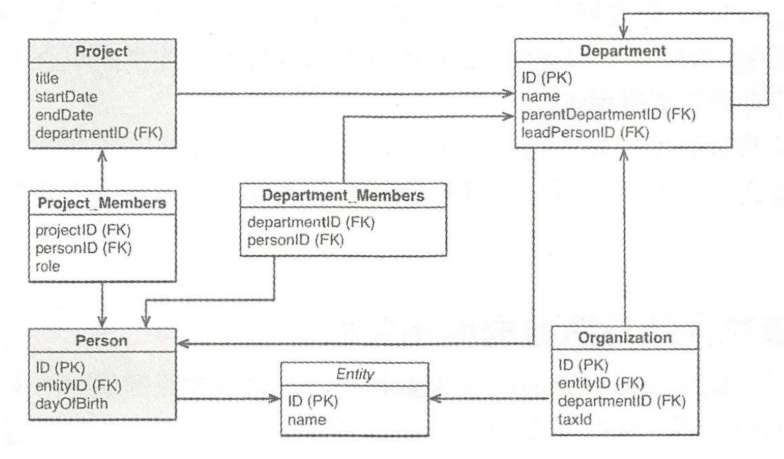
\includegraphics[width=\textwidth]{images/14.png}
    \caption{关系型数据库}
    \label{fig:relational}
	\end{subfigure}

	\begin{subfigure}[b]{1\textwidth} 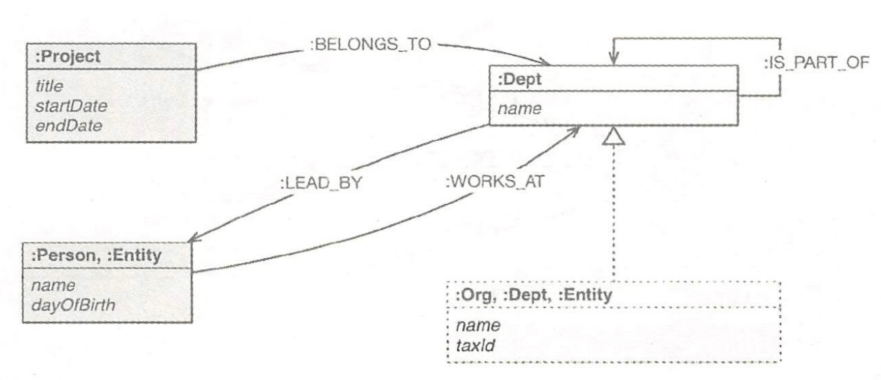
\includegraphics[width=\textwidth]{images/15.png}
    \caption{图数据库}
    \label{fig:graph_db}
	\end{subfigure}
	\caption{关系型数据库和图数据库的对比}
	\label{fig:relational_vs_graph}
\end{figure}


与此同时, NoSQL数据库的兴起为解决结构化与非结构化数据存储问题提供了多样化的方案, 其中图数据库因其高效管理和存储关联关系数据的特性而受到关注. 与其他类型的NoSQL数据库 (如键值数据库、文档数据库) 相比, 图数据库的优势在于其在图结构上的高效性和灵活性, 能够处理关系紧密的数据集. 图数据库通过将实体 (节点) 和实体之间的关系 (边) 作为“一等公民”进行管理, 极大简化了复杂关联查询的实现.

此外, 社交网络、知识图谱、推荐系统等应用的普及也是图数据库迅速发展的重要驱动力, 因为这些领域的数据模型本质上是高度关联的网状结构, 图数据库在这些场景下具备显著的优势, 可以高效地表达、存储和查询数据中的复杂关系, 如\cref{fig:graph_db}所示. 因此, 图数据库逐渐被应用于越来越多的场景, 并成为处理关联数据的核心工具.

图数据库的发展分为几个阶段, 最初的Graph1.0阶段是基于小规模原生图存储, 代表性产品是Neo4j的早期版本, 其主要存储规模限制在百万级节点和边. 随着大数据时代的到来, Graph2.0阶段的图数据库支持分布式存储和计算, 使得它们能够应对大规模的数据集, 例如JanusGraph和TigerGraph等, 实现了数十亿节点和边的存储与管理, 并显著提升了系统的扩展性和容错能力. 近年来, Graph3.0阶段的图数据库产品开始强调实时性和高并行计算能力, 进一步提升了查询性能, 使得实时复杂查询和分析成为可能, 同时支持更加复杂的计算任务的并行化处理, 例如内置的图算法库和支持多线程的并行计算.

\clearpage % 确保清理所有浮动内容